\section{Case Study}
\label{sec:case_study}
In this section, we present three case studies for our system covering different types of events including the Chardon High School Shooting, 
the Occupy Wall Street protests in New York, and the 2011 Virginia Earthquake. 
The first case shows how analysts can use our system efficiently to find and explore an abnormal event.
The second case highlights the differences between social media types by cross validation of a planned event.
Finally, the last example showcases the effects of an abrupt, unexpected, natural disaster.

%\begin{figure*}[t]
	%\centering
	%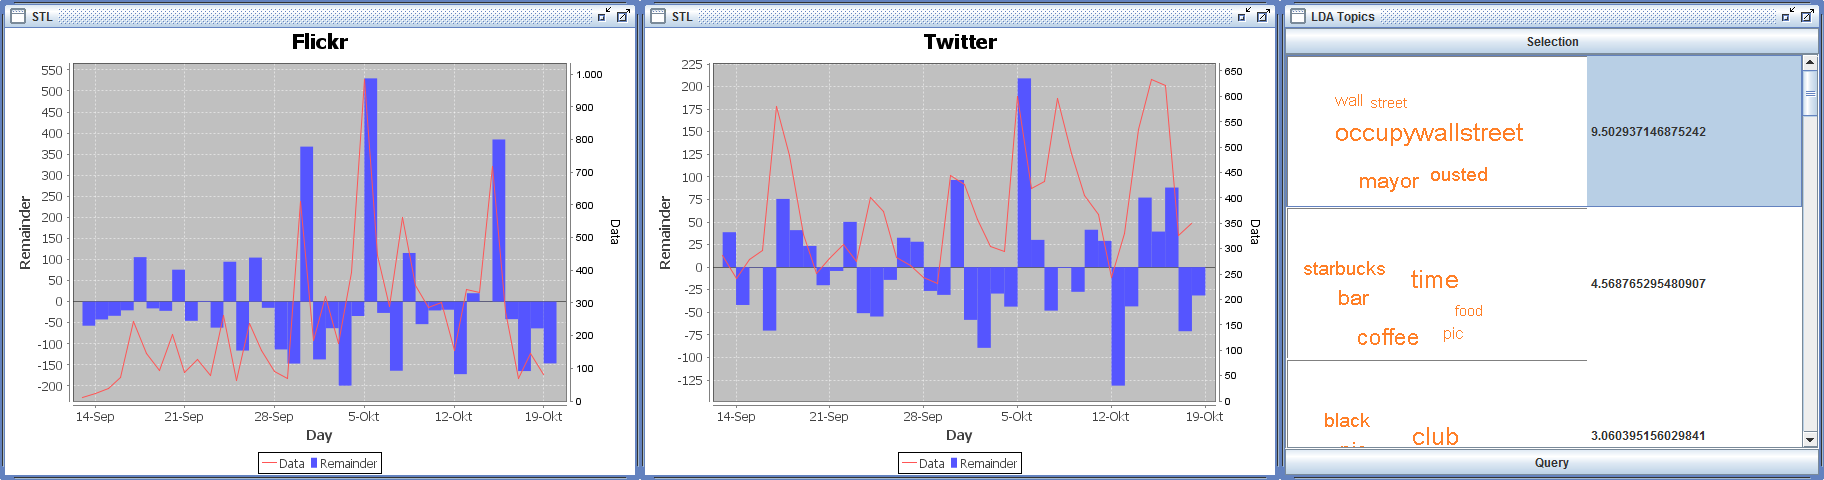
\includegraphics[width=1.00\linewidth]{images/flickrtwitter}
	%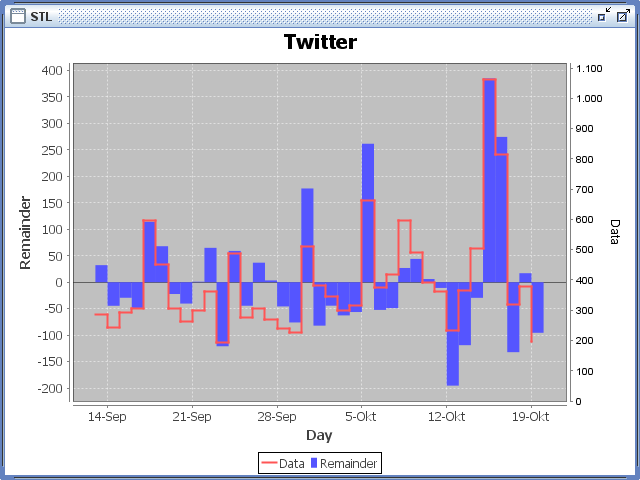
\includegraphics[width=0.45\linewidth]{images/twitter_wallstreet.png}
	%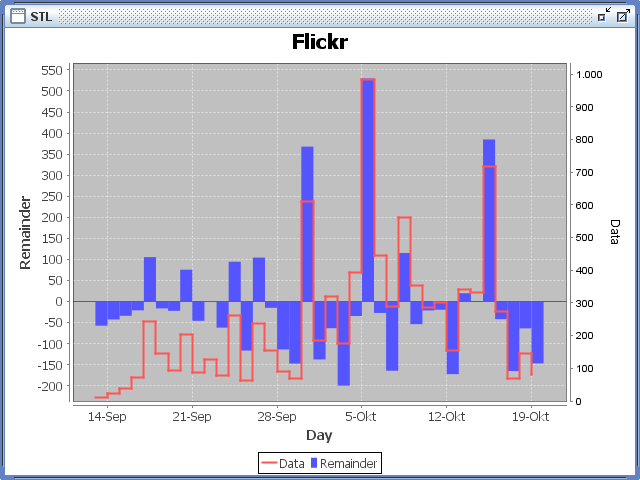
\includegraphics[width=0.45\linewidth]{images/flickr_wallstreet.png}
	%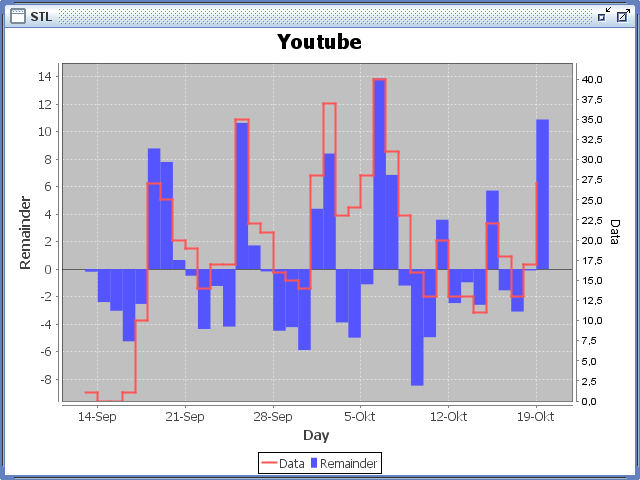
\includegraphics[width=0.45\linewidth]{images/occupyyoutube.png}
	%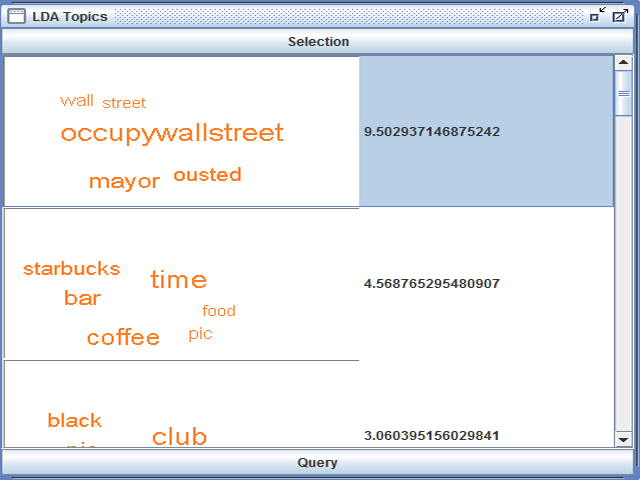
\includegraphics[width=0.45\linewidth]{images/tags_wallstreet.png}
	%\caption{Cross validation of an event using Twitter, Flickr, and YouTube data for the Occupy Wall Street Protests.
	%The protests occurred on Sep. 17 and 30, Oct. 5 and 15. The extracted topics from messages using LDA are displayed with the z-score
	%on the right. The line charts show the remainder components $R_{t}$ (blue) and the original data volumes $Y_{t}=ts_i$ (red) for the STL evaluation.}
	%\label{fig:wallstreet}
%\end{figure*}
	

\subsection{Ohio High School Shooting}
\label{subsec:ohio_shooting}
On February 27, 2012, a student opened fire inside the Chardon High School cafeteria in the early morning.
The gunman killed one student and injured four, from which two eventually died after the incident.

To examine this incident we first locate and select the broader Cleveland area on the map and select a time frame covering three days from February 26 to February 28. 
Using the text search engine and a wildcard query (\textquoteleft *\textquoteright) we can establish an exploration context showing all messages plotted on the map with their respective contents and meta data listed in a separate table view. First, we want to get a broad overview of the topics discussed in the region and thus we select all messages in the area and apply the LDA extraction tool to the current selection. In order to see the most general topics, we chose a low parameter value for the number of topics and a high iteration count to achieve good separation. At this level of semantic detail, the extracted topics indicate messages about the NBA all-star game (February 26 in Orlando) with keywords like \textit{kobe, game, dunk and lebron} as well as the showing of the movie \textquoteleft The Lion King\textquoteright on TV with keywords \textit{king, lion, tv}. If we look at the STL-Diagrams of these topics and the computed z-scores, we also see a peak for these events. By clicking on the retrieved topic representations the associated messages are highlighted in each view. By reading some of the message contents (e.g. \textit{'Watching my fav. Movie on ABC family..... Lion King!!!!', 'Can't wait till the dunk contest starts!'}), the analyst can easily disqualify these from further analysis.

To get a higher semantic resolution we can now increase the number of topics and slightly decrease the iteration count in order to achieve a fast computation. By selecting 20 topics, the topic indicating the shooting event is extracted and indicated by keyterms like \textit{shooting, chardon and school}, alongside the other topics. Although the proportion of the topic is not very high compared to the others, the topic receives a very high z-score (i.e., 3.77) and is ranked among the top five topics (highlighted in orange). Figure~\ref{fig:system} demonstrates the system view of this observation. An analyst can now select the incident topic to see the spatial distribution of associated messages on the maps as well as the temporal distribution in the timeslider histogram. By examining messages using the content lens to aggregate topics over map areas as well as the tools for reading individual message contents, we can easily distinguish between messages informed by media reaction and messages of actual observers in the Chardon High School area. In this case, after isolating the messages from local observers, we find messages like \textit{\textquoteleft Omg shooting at Chardon High School?!?!\textquoteright} and \textit{\textquoteleft Helicopter overhead. We are on scene. Message from school says students moved to middle school\textquoteright}.

\begin{figure}[tb]
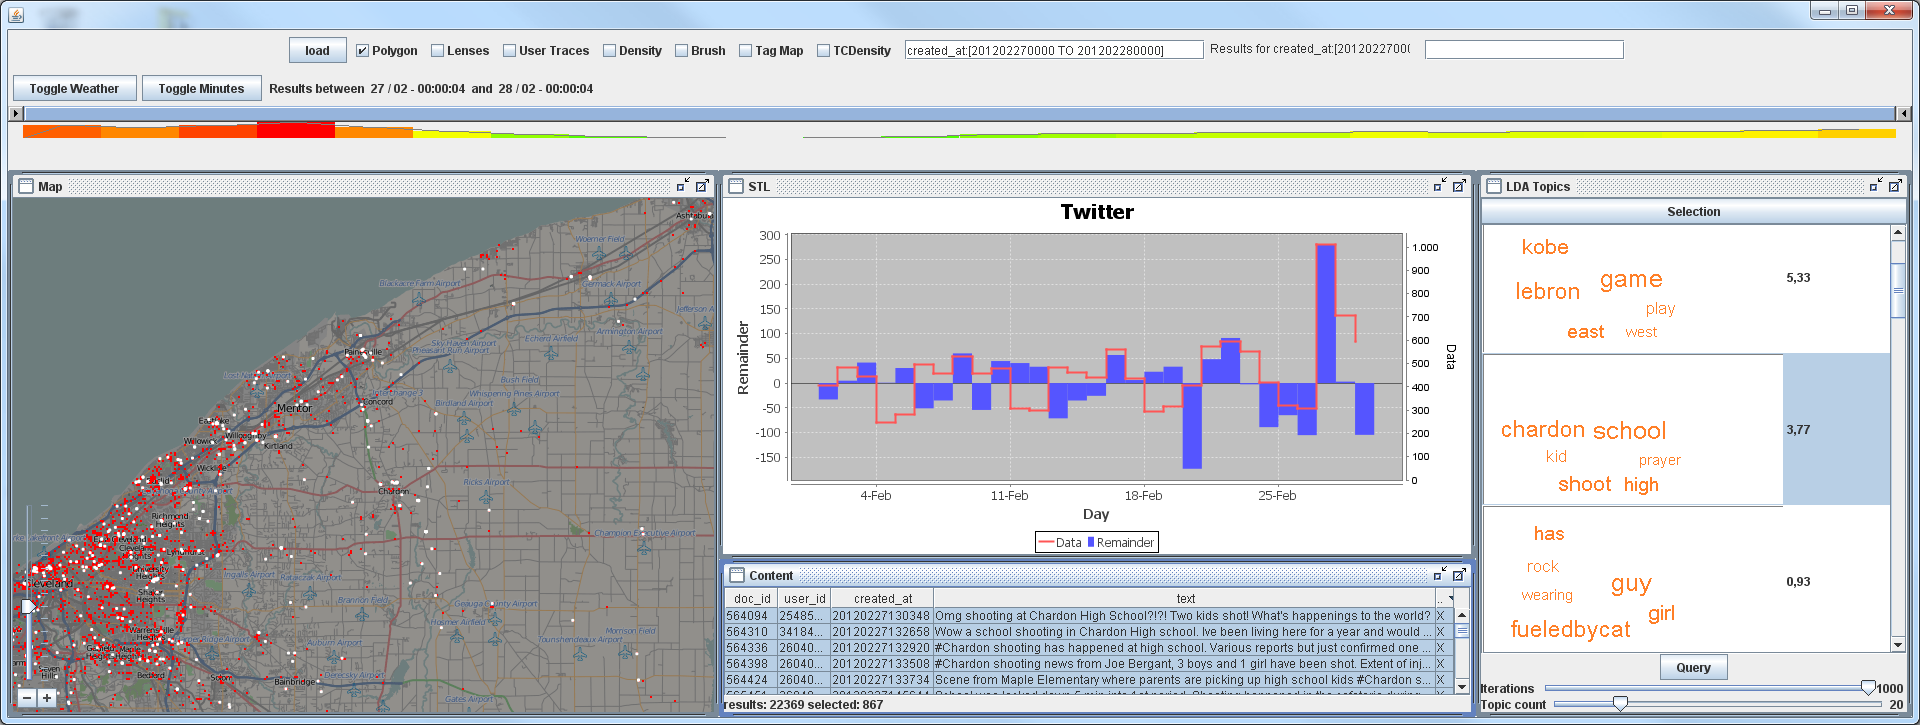
\includegraphics[width=1.0\linewidth]{teaser}
\caption{Social media analysis system including message plots on a map, abnormality estimation charts and tables for message content and topic exploration. 
  It can be seen, how the Ohio High School Shooing on February 27, 2012 is examined using the system. The selected messages, marked as white dots on the map, show retrieved Tweets that are related to the event.}
\label{fig:system}
\end{figure}



%To discussion -> Athough the detected messages could help to identify local witnesses of some event, the frequencies of messages with geocoordinates are still very low in moderately populated areas ---- daher könnte man die Nützlichkeit zum gegenwärtigen Zeitpunkt sicher hinterfragen...

%\footnote{\url{http://www.cbsnews.com/8301-504083_162-57386775-504083/third-chardon-high-school-shooting-victim-demetrius-hewlin-dies/}}

\subsection{Occupy Wall Sreet}
\label{subsec:occupy_wallst}

Starting on September 17, 2011 in the Wall Street financial district in New York City,
people have been gathering for the Occupy Wall Street protest movement.
The movement against economic inequality has since spread to other major cities throughout the world.
Various social media services including Twitter, Facebook, Flickr and Youtube have been utilized both by the participants and the global media for communication and reports about the movement in forms of text, images and videos. 
For the related extracted topic (\textit{occupywallstreet, wall, takewallstreet, takewallst, park}), 
Figure~\ref{fig:wallstreet} shows the results of our abnormality estimation for the three social media services Twitter, Flickr, and YouTube over the course of one month.
As shown in Figure~\ref{fig:plot}, in each of the marked regions, at least two of the services show z-scores over 2.0 and they correspond to actual events during the Occupy Wall Street protests.
From this experimental result, one can derive a strong correlation between the three social media data sources.
The related data volumes and remainder ($R$) are shown in Figure~\ref{fig:wallstreet} for all three providers.

\begin{figure}[tb]
\centering
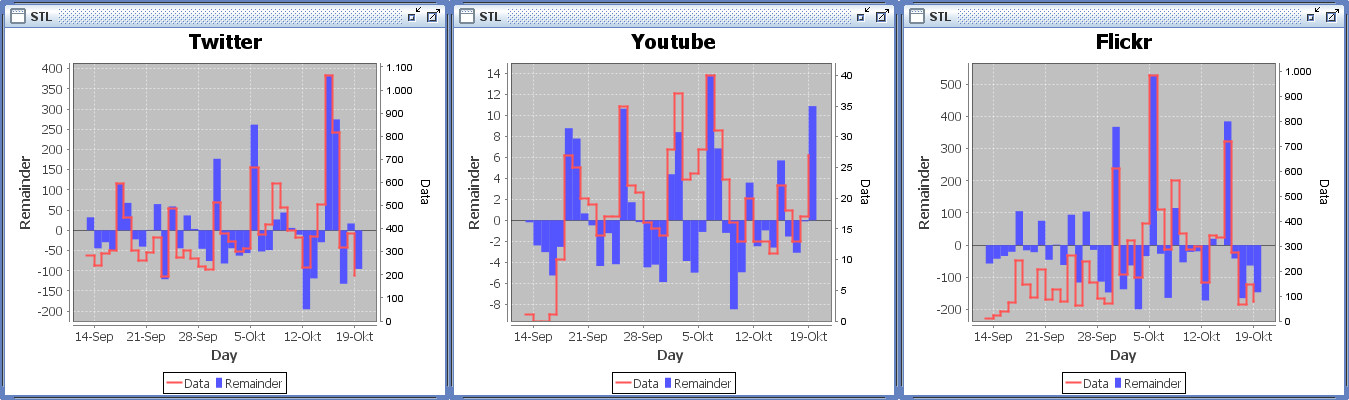
\includegraphics[width=1.0\linewidth]{crosscompare_new}
\caption{Cross validation of an event using Twitter, Flickr, and YouTube data for the Occupy Wall Street Protests.
	The protests occurred on Sep. 17 and 30, Oct. 5 and 15. The line charts show the remainder components $R$ (blue) and the original data volumes $Y$ (red) for the STL evaluation. The scales on the right and left side of each chart view are adapted to the maximum values.}
\label{fig:wallstreet}
\end{figure}


\begin{figure}[tb]
\centering
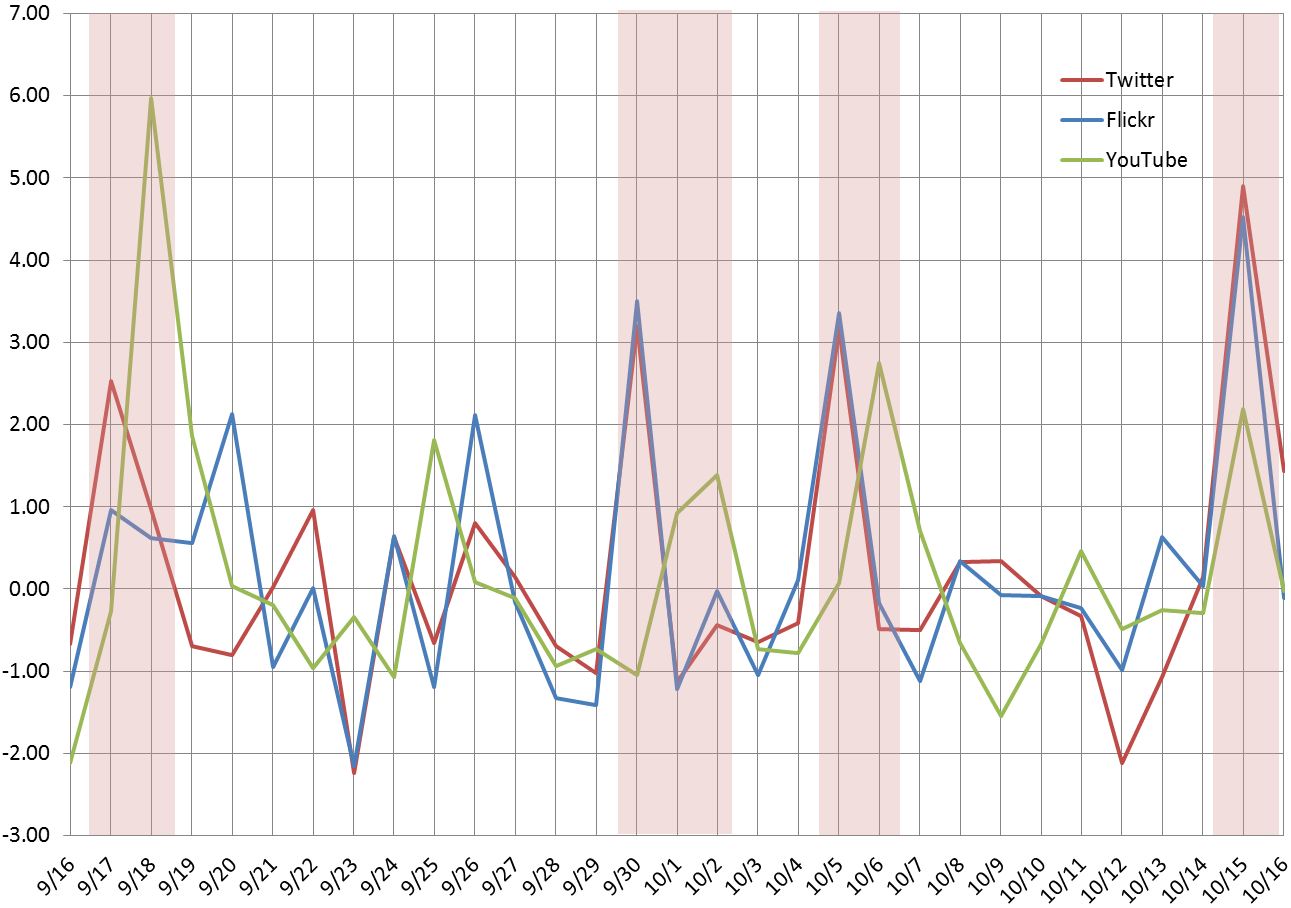
\includegraphics[width=0.8\linewidth]{z-score-plot}
\caption{Abnormality and correlation on multiple social media sources. 
As a result of high z-scores around the same time periods, we found a strong correlation 
between the three social media sources. Marked regions correspond to periods where at least 2 providers received scores over 2.0.}
\label{fig:plot}
\end{figure}



As shown in Figure~\ref{fig:plot}, on September 17 (the first day of the protests with approximately 1,000 participants~\cite{Sept17}),
only the Twitter stream received an abnormal score while the Flickr and YouTube data artifacts are delayed by 1-3 days.
We attribute this initial delay to the simple nature of Twitter usage compared to Flickr and YouTube where the data potentially has to be recorded, edited, and uploaded and is thus more labor intensive.
Additionally, eighty protesters where arrested while marching uptown on September 24, but even though Flickr and YouTube reaction on this event created higher z-scores in the following days, they were not significant enough to register an event.
The following spikes of high z-scores overlap with a march across the Brooklyn Bridge (Oct. 1~\cite{Oct01}), a large demonstration (Oct. 5~\cite{Oct05}), and globally coordinated protests (Oct. 15~\cite{Oct15}).

%For YouTube, the high abnormalities usually come with a delay between one and two days.
%Our system found the additional abnormal events \textit{oakland, tear, gas, general, san}~\cite{Duell:2011:OOI} and \textsl{bridge, brooklyn, arrests, march, police}~\cite{Chiaramonte:2011:CMO} in the YouTube meta-data, which were not detectable in Twitter and Flickr.
%Our system also provides further analysis on YouTube data. 
%We applied our abnormality estimation method to meta-data from YouTube. 
%Our system additional found more abnormal events;

%%
%% Table of experimental results of topic model
%%
%\begin{table}\footnotesize
%\begin{table}
%\small
%\centering
%\begin{tabular}{|l|c|c|c|}
%	\hline
%	 Date & Twitter & Flickr & YouTube \\
%	\hline\hline
%%	Sep. 16, 2011 & -0.67 & -1.19 & -2.12 \\
%	Sep. 17, 2011 & \textbf{2.53} & \textbf{0.97}& \textbf{-0.26} \\ %& The protests movement began \\
%	Sep. 18, 2011 & 0.97 & 0.62 & 5.98 \\ 
%	Sep. 19, 2011 & -0.69 & 0.56 & 1.86 \\
%	Sep. 20, 2011 & -0.80 & 2.13 & 0.04 \\
%	Sep. 21, 2011 & 0.02 & -0.95 & -0.19 \\
%	Sep. 22, 2011 & 0.96 & 0.01 & -0.96 \\ 
%	Sep. 23, 2011 & -2.24 & -2.15 & -0.34 \\
%	Sep. 24, 2011 & 0.63 & 0.64 & -1.07 \\
%	Sep. 25, 2011 & -0.66 & -1.19 & 1.81 \\
%	Sep. 26, 2011 & 0.80 & 2.11 & 0.08 \\
%	Sep. 27, 2011 & 0.14 & -0.16 & -0.11 \\
%	Sep. 28, 2011 & -0.70 & -1.32 & -0.94 \\
%	Sep. 29, 2011 & -1.02 & -1.41 & -0.73 \\
%	Sep. 30, 2011 & \textbf{3.20} & \textbf{3.50} & -1.05 \\%& Big movement \\
%	Oct. 1, 2011 & -1.14 & -1.22 & 0.92 \\
%	Oct. 2, 2011 & -0.44 & -0.03 & \textbf{1.38} \\
%	Oct. 3, 2011 & -0.64 & -1.05 & -0.73 \\
%	Oct. 4, 2011 & -0.42 & 0.11 & -0.77 \\
%	Oct. 5, 2011 & \textbf{3.17} & \textbf{3.36} & 0.07 \\ %& Unions, students join the protest\\
%	Oct. 6, 2011 & -0.49 & -0.18 & \textbf{2.75} \\
%	Oct. 7, 2011 & -0.50 & -1.12 & 0.7 \\
%	Oct. 8, 2011 & 0.32	& 0.34 & -0.65 \\
%	Oct. 9, 2011 & 0.34	& -0.07 & -1.54 \\
%	Oct. 10, 2011 & -0.09 & -0.08 & -0.67 \\
%	Oct. 11, 2011 & -0.33 & -0.23 & -0.46 \\
%	Oct. 12, 2011 & -2.12 & -0.99 & -0.49 \\
%	Oct. 13, 2011 & -1.07 & 0.63 & -0.26 \\
%	Oct. 14, 2011 & 0.15 & 0.04 & -0.3 \\
%	Oct. 15, 2011 & \textbf{4.90} & \textbf{4.53} & \textbf{2.19} \\ %& Global day of action \\
%%	Sep. 17, 2011 & 2.53 & 0.97 & Sep. 18, 2011 & 5.98 \\ %& The protests movement began \\
%%	Sep. 30, 2011 & 3.20 & 3.50 & Oct. 2, 2011 & 1.38 \\%& Big movement \\
%%	Oct. 5, 2011 	 & 3.17	& 3.36 & Oct. 6, 2011 & 2.75 \\ %& Unions, students join the protest\\
%%	Oct. 15, 2011   & 4.90 & 4.53 & Oct. 15, 2011 & 2.19 \\ %& Global day of action \\
%	\hline
%\end{tabular}
%\caption{Abnormality and correlation on multiple social media. 
%As a result of the high z-scores around the same time, we found a strong correlation 
%between the three social media sources.}
%\label{T:Correlation}
%\end{table}
%\footnote{\url{http://www.nytimes.com/2011/11/25/business/media/occupy-movement-focuses-on-staying-current-on-social-networks.html}}

%\subsection{2011 Virginia earthquake}
%\label{subsec:virginia_earthquake}
%A magnitude 5.8 earthquake occurred on August 23 afternoon, 2011 in Mineral, Virginia,
%according to the U.S. Geological Survey\footnote{\url{http://earthquake.usgs.gov/earthquakes/recenteqsww/Quakes/se082311a.php}}.
%During and after the tremors were felt along the East Coast,
%Twitter users posted more than 40,000 earthquake-related reaction tweets
%within a minute of its occurrence\footnote{\url{http://mashable.com/2011/08/23/virginia-earthquake/}}.
%There are some example Twitter messages;
%\textit{EARTHQUAKE!!!!!!!}; \textit{Whoa!!!! Just experienced an earthquake here in Virginia!!!!}; 
%\textit{Omg I just felt an earthquake}.
%Using our method, we found also the z-score of the topic indicating the earthquake event was 
%extremely high (i.e., 10.63).
\subsection{2011 Virginia Earthquake}
\label{subsec:virginia_earthquake}
For the last use case we examine a magnitude 5.8 earthquake that occurred on the afternoon of August 23rd 2011 in Mineral, Virginia~\cite{USGS:2011:M5V}.
%\footnote{\url{http://earthquake.usgs.gov/earthquakes/recenteqsww/Quakes/se082311a.php}}.
Starting with the minute of the earthquakes occurrence, Twitter users posted more than 40.000 earthquake-related Tweets reporting tremors they felt along the East Coast~\cite{Indvik:2011:ECT}.
%\footnote{\url{http://mashable.com/2011/08/23/virginia-earthquake/}}.
Among these were messages like:
\textit{\textquoteleft EARTHQUAKE!!!!!!!\textquoteright}; \textit{\textquoteleft Whoa!!!! Just experienced an earthquake here in Virginia!!!!\textquoteright}; and 
\textit{\textquoteleft Omg I just felt an earthquake\textquoteright}.
Figure~\ref{fig:earthquake} gives an impression how our system is applied to examine this event.

\begin{figure}[htb]
	\centering
	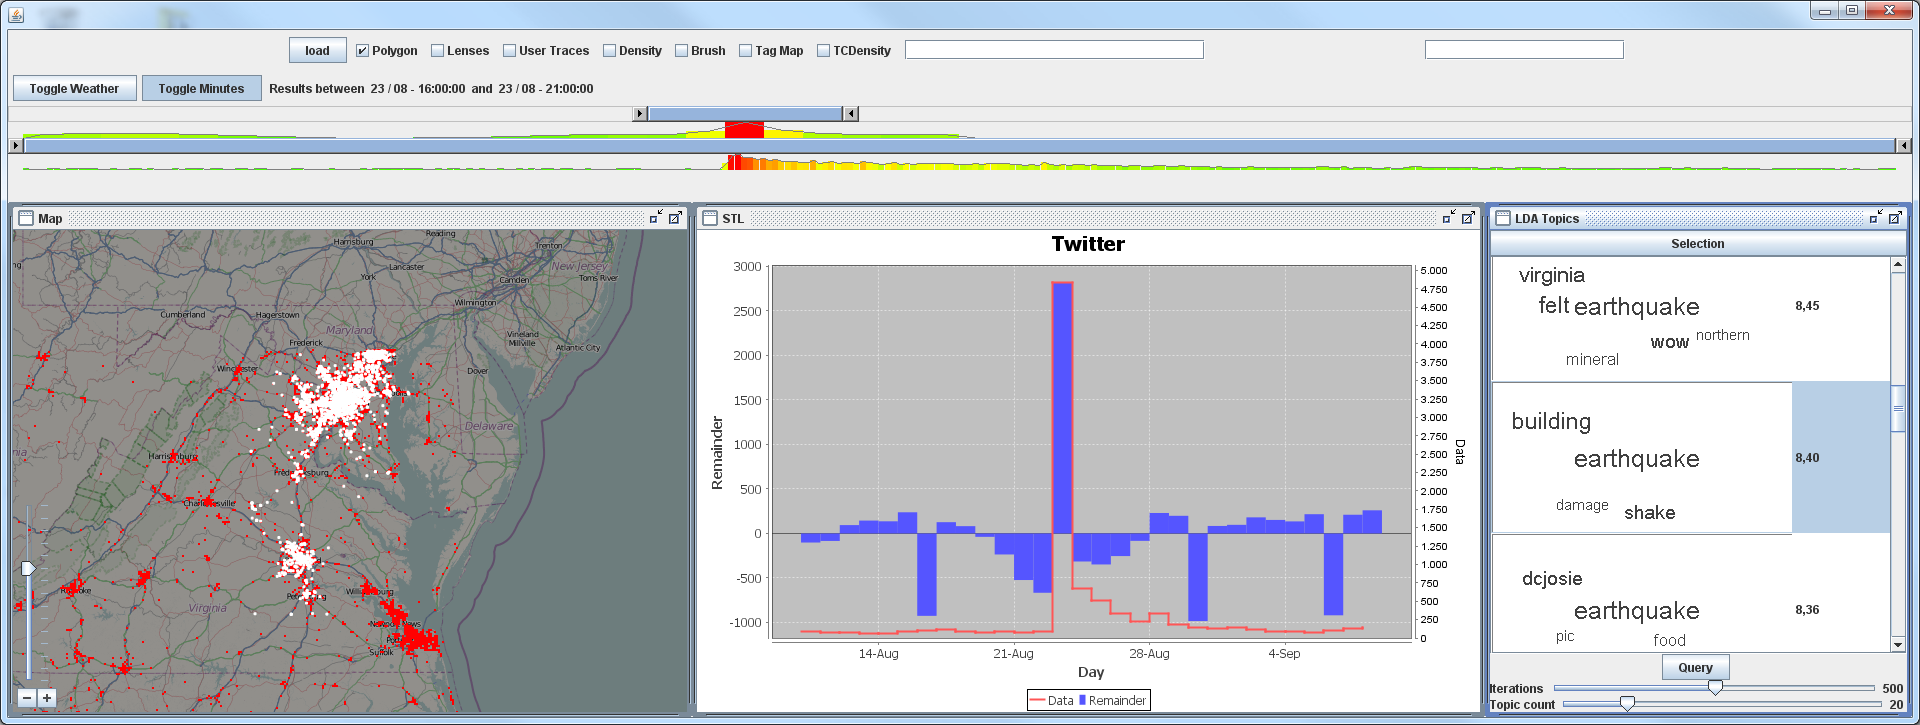
\includegraphics[width=1.0\linewidth]{earthquake3}
	\caption{Virginia earthquake on August 23rd, 2011. Our abnormal event detection system detects the earthquake event
	using our STL based anomaly detection algorithm. The abnormality degree is extremely high
	on August 23rd, 2011 (times are given in UTC).}
	\label{fig:earthquake}
\end{figure}

For the analysis we begin with selecting the Virginia area from Baltimore to Virginia Beach and three days around the 23th. A topic extraction with 5 topics and just 100 iterations already retrieves two earthquake related topics showing that this event is very prominent within the selection. By clicking these topics one can observe that the highest density of earthquake messages can be found in the Washington, Baltimore and Richmond areas. 

To observe the areas in more detail we combine the topic selection with a spatial selection of the three cities and reapply the topic extraction. This time we use 20 topics with 500 iterations. Since we are now operating only on earthquake related messages, the retrieved topics all contain earthquake as a dominant keyword. On this level of detail we can see topics indicating that buildings have been evacuated due to the earthquake (\textit{earthquake, people, evacuated, early, building}) and that damage has been caused (\textit{earthquake, building, shake, damage}). The z-scores for all top ranked topics are now very high (often above 8.0) and thus indicate the high abnormality of this event. 

Finally, when going into even higher detail with 100 topics and 1000 iterations we can see smaller events within the big earthquake event. For example, one topic indicates that damage was caused to the Washington Monument and by clicking on the topic we can see messages like \textit{\textquoteleft damage to Washington Monument\textquoteright}; \textit{\textquoteleft Washington Monument is tilting?!? \textquoteright}; and \textit{\textquoteleft Helicopter just landed next to Washington Moniment, west side. \#DCearthquake \textquoteright}. There are also misleading messages, indicating that the damage to the Washington Monument was just false rumors: \textit{\textquoteleft the Washington monument was not damaged in any way from the earthquake. \#rumor\textquoteright}. However, media crosschecks show that visible damages did in fact happen and will probably cost the city 15 million dollars to repair~\cite{Huffingtonpost:2012:Web}.

At this point, it is important to note, that while several earthquake topics produced significant z-values in Twitter, the event did not produce high z-scores in Flickr and YouTube.
This is probably due to fact, that many people will write a quick message after a shock has been felt by themselves, but it takes quite some time until images or videos are uploaded from cameras to Flickr and YouTube. The event also demonstrates that large and unexpected events will produce immediate and significant reactions in services like Twitter and they can thus easily be detected by using our system.
